\subsection{Динамический режим}
С помощью осциллографа снимем ВАХ тиратрона в динамическом режиме при двух
значениях напряжений накала лампы: \\$V_1^{нак} = 2,830\pm 0,001$ В, $V_2^{нак} = 3,392 \pm 0,001$ В.
По полученной на экране осциллографа ВАХ определим $V_{мин}$, $V_{макс}$, 
$V_{проб}$. Занесём результаты измерений в таблицу:

\begin{table}[h!]
  \centering
  \caption{Измерения в динамическом режиме}
  \begin{tabular}{|c|c|c|c|c|}
    \hline
    № & $V_{нак}$, В & $V_{макс}$, В & $V_{мин}$, В & $V_{проб}$, В \\ 
    \hline
    1 & $2.830 \pm 0.001$ & $ 5.4 \pm 0.4$ & $ 10.4 \pm 0.4$ & $11.7 \pm 0.4$ \\ \hline
    2 & $3.392 \pm 0.001$ & $6.2 \pm 0.4$   & $ 9.8 \pm 0.4$    &  $ 11.5 \pm 0.4$ \\ 
    \hline
  \end{tabular}
\end{table}

Приняв $U_0 = 2.5$ эВ, рассчитаем размер электронной оболочки атома инертного
газа по формулам, заполняющего лампу по формулам
\eqref{eq::first_max_cond}-\eqref{eq::l_3}. Предварительно оценим погрешности
как:
\[
  \sigma_{l_1} = l_1 \cdot \frac{\sigma_{E_1}}{E_1} 
  \: 
  \sigma_{l_2} = l_2 \cdot \frac{\sigma_{E_2}}{E_2}
  \: 
  \sigma_{l_3} = l_3 \cdot \frac{\sigma_{E_2} - \sigma_{E_1}}{E_2 - E_1}
\]
Погрешность глубины потенциальной ямы из формулы \eqref{eq::Umin}:
\[
  \sigma_{U_0} = \frac{4}{5} E_2 + \frac{9}{5} E_1
\]
\begin{table}[h!]
  \centering
  \caption{Рассчёт размера оболочки атома}
  \begin{tabular}{|c|c|c|c|c|}
    \hline
    № & $V_{нак}$, В & $l_1$, \AA & $l_2$, \AA & $l_3$, \AA \\ 
    \hline
    1 & $2.830 \pm 0.001$ & $2.2 \pm 0.2$ & $ 2.6 \pm 0.1$ & $3.1 \pm 0.5$ \\ \hline
    2 & $3.392 \pm 0.001$ & $2.1 \pm 0.1$ & $ 2.6 \pm 0.1$ & $ 3.6 \pm 0.8$ \\ 
    \hline
  \end{tabular}
  \begin{tabular}{|c|c|c|c|}
    \hline
    № & $V_{нак}$, В & $\overline{l}$, \AA & $U_0^{эксп}$, эВ\\
    \hline
    1 & $2.830 \pm 0.001$ & $2.6 \pm 0.3$ & $ 1.4 \pm 1.0$\\\hline
    2 & $3.392 \pm 0.001$ & $2.8 \pm 0.3$ & $ 3 \pm 1$\\
    \hline
  \end{tabular}
\end{table}
Усредним значения в таблице и получим:
\[
  U_0^{эксп} = 2.2 \pm 1 \: \text{эВ}
\]
\[
  l = 2.7 \pm 0.3 \: \text{\AA}
\]
Сравнивая с теорией $U_0 = 2.5$ эВ и $l^{теор} = 2.8 \pm 0.1$ \AA, заметим, что
результаты совпадают в пределах погрешности. В качестве табличного значения $l$
был выбран удвоенный радиус ксенона, так как в эксперименте пробой наблюдался
при $E = 11.6 \pm 0.4$ эВ, что достаточно близко к энергии ионизации ксенона
$12.1$ эВ.

\subsection{Статический режим}

По результатам измерений в статическом режиме построим ВАХ тиратрона для
значений $V_1^{накала} = 2.837 \pm 0.001$ В и $V_2^{накала} = 3.402 \pm 0.001$
В, а также отметим на них точки максимума и минимума. Построим также график
зависимости вероятности $w$ рассеяния электрона атомом ксенона от напряжения на
катоде $V$ по формуле \eqref{eq::probability} (с точностью до константы), основываясь на ВАХ для $V_1^{накала} =
2.837 \pm 0.001$.

\begin{figure}[h!]
  \centering
  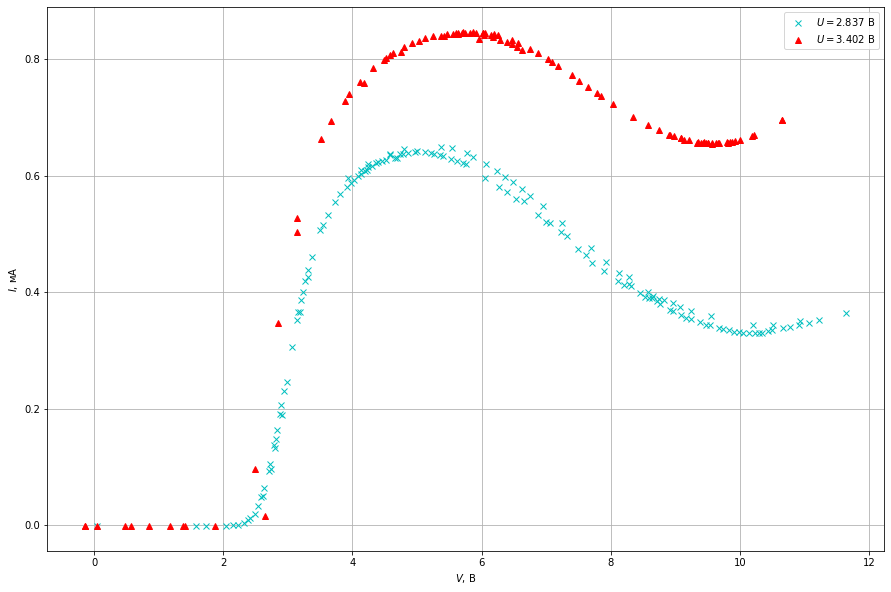
\includegraphics[width=0.9\linewidth]{VAH.png}
  \caption{ВАХ тиратрона для двух значений напряжения накала}
  \label{img::VAH}
\end{figure}
\begin{figure}[h!]
  \centering
  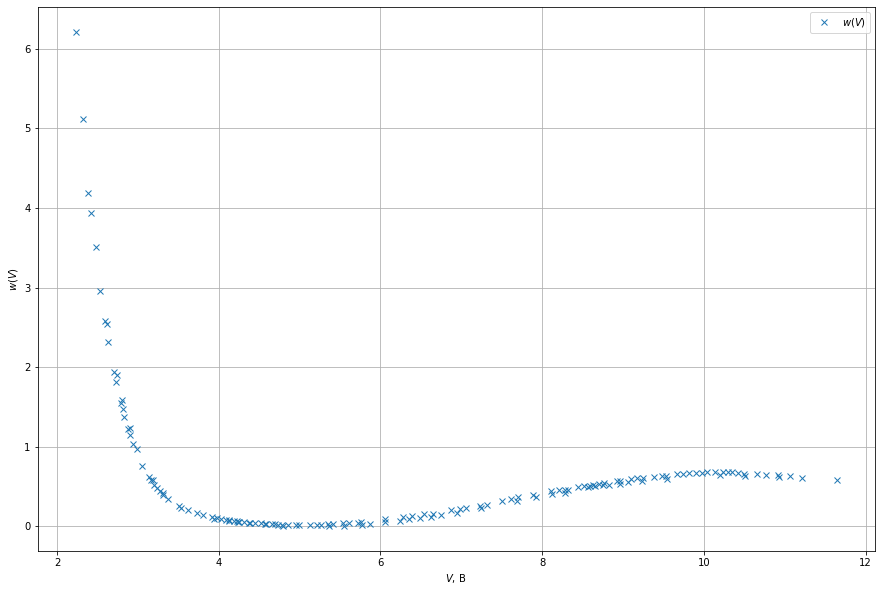
\includegraphics[width=0.8\linewidth]{wU.png}
  \caption{Характер зависимости вероятности рассеяния электрона атомом ксенона от напряжения на катоде}
\end{figure}

Из графика \ref{img::VAH} видно, что точки максимумов и минимумов совпадают с
измеренными ранее (в динамическом режиме).

Используя формулу \eqref{eq::max_cond}, оценим, при каких напряжениях должны
появляться максимумы в коэффициенте прохождения электронов для $n = 2, 3$,
предварительно выразив из неё $E_n$:
\[
  E_n = n^2 \left(E_1 + U_0\right) - U_0
\]
Получим для $n = 2, 3$:
\[
  E_2 = 29.1 \: \text{эВ} \quad
  E_3 = 68.6 \: \text{эВ}
\]
Полученные значения выше потенциала ионизации, поэтому эти максимумы уже не
будут наблюдаться.

\section{Вывод}

В ходе работы была исследована ВАХ тиратрона двумя методами: статическим и
динамическим. В обоих случаях результаты оказались близки к теории. Было
получено значение размера внешней оболочки атома инертного газа тиратрона и
потенциал его ионизации, по которому было определено, что данный газ есть
ксенон. Также был получен характер зависимости вероятности рассеяния электрона
атомом ксенона  в зависимости от напряжения на катоде.